\section{Nombre: Quetzalcóatl}  \label{per:quetzalcoatl}
\subsection{Descripción:}
Quetzalcóatl es descrito como un dios blanco y barbado pero nadie lo ha visto después de que decidiera exiliarse.
\subsection{Status:}
\begin{itemize}
		\item Personaje no jugable.
	\end{itemize}
\subsection{Imagen}
Ver figura \ref{fig:quetDiseno}
	\begin{figure}
					\centering
					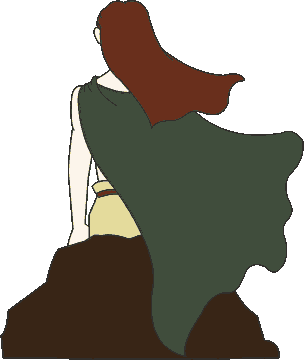
\includegraphics[height=0.3 \textheight]{Imagenes/quet}
					\caption{Concepto de diseño de Quetzalcóatl.}
					\label{fig:quetDiseno}
	\end{figure}
\subsection{Concepto:}
\begin{itemize}
	\item \textbf{Historia antes del juego:}
	Dios que tras perder la batalla de Tula contra Tezcatlipoca decide autoexiliarse. Los dioses que le juraron lealtad cuando se creo el quinto sol esperan su retorno.
	\item \textbf{Historia durante el juego:}
	Al encontrarse exiliado no participa directamente en la historia pero se le ha visto en la caída de Tenochtitlan.
\end{itemize} 
\subsection{Encuentro:}
Se le ve por primera y única vez en la cinemática 1.
\subsection{Habilidades:}
Dios de gran poder capaz de derrotar a Tezcatlipoca si ayuda. Se sabe que ha sido capaz de destruir mundo enteros así como crearlos
\subsection{Armas:}
Sin armas confirmadas.
\subsection{Ítems:}
Se sospecha que tiene en su poder muchas armas de carácter legendario.
\subsection{Bloques de animación:}
	\begin{itemize}
		\item Animación sentado.
	\end{itemize}